\icode{E-MI-SI-L2-261104-001}
在竖直平面内的半圆环上，两根等长的细线\(AO\)、\(BO\)结于圆心\(O\)，下悬重为\(G\)的物体。现使\(AO\)线固定，\(BO\)线的\(B\)端沿圆环从位置\(C\)逐渐滑至\(D\)，则\(AO\)、\(BO\)中的拉力\(F_A\)、\(F_B\)的变化情况是\paren[]

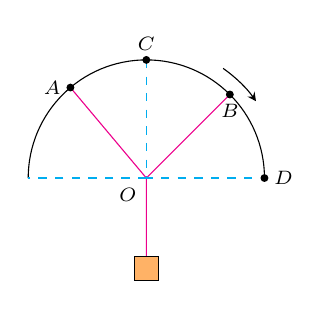
\begin{tikzpicture}[>=stealth,font=\scriptsize]
	\draw (1.5,0)node[right]{\(D\)} arc (0:180:1.5);
	\draw[magenta] (130:1.5)node[left,black]{\(A\)}--(0,0)--(0,-1) (45:1.5)node[below,black]{\(B\)}--(0,0)node[below left,black]{\(O\)};
	\draw[dashed,cyan] (0,1.5)node[above,black]{\(C\)}--(0,0)--(1.5,0) (0,0)--(-1.5,0);
	\draw[->] (55:1.7) arc(55:35:1.7);
	\foreach \r in {130,90,45,0}
		\fill (\r:1.5) circle(.05);
	\draw[fill=orange!60] (-.15,-1) rectangle(.15,-1.3);
\end{tikzpicture}
\begin{choices}
	\item\(F_A\)不变，\(F_B\)变大
	\item\(F_A\)变大，\(F_B\)先变小后变大
	\item\(F_A\)变大，\(F_B\)先变大后变小
	\item\(F_A\)、\(F_B\)都变大
\end{choices}
\begin{answer}
	B\qquad 提示：受力分析并构建力的矢量三角形
	
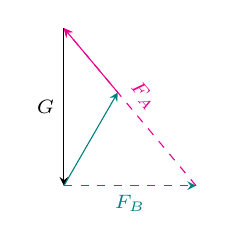
\begin{tikzpicture}[>=stealth,font=\scriptsize]
	\draw[->] (0,0)--node[left]{\(G\)}(0,-2);
	\draw[->,dashed,teal] (0,-2)--node[below]{\(F_B\)}({2*tan(40)},-2);
	\draw[->,dashed,magenta] ({2*tan(40)},-2)--node[above,rotate=-50]{\(F_A\)}(0,0);
	\draw[->,teal] (0,-2)--++(60:{4*tan(40)/(1+sqrt(3)*tan(40))})coordinate(f);
	\draw[->,magenta] (f)--(0,0);
\end{tikzpicture}
\end{answer}